\newpage
\fancyhf{}
\lhead{Silas Leidel}
\rhead{Seite \thepage}

\section{Wasserversorgung}

\subsection{Planung/ Realisation}
Da das Projekt für Beete und Töpfe geplant ist, ist die benötigte Wassermenge pro einmaliger
Wässerung und über einige Zyklen überschaubar.Am Beispielfall der Orchidee, eine der beliebtesten
Zimmerpflanzen in Deutschland, wird
der Wasserverbrauch verdeutlicht. Eine Orchidee sollte im Sommer zweimal wöchentlich gegossen werden.
 Bei jedem Gießvorgang werden ca. 100ml Wasser verbraucht. Bei drei Pflanzen liegt der Wasserverbrauch
 bei 600ml in der Woche. Die meisten
anderen beliebten Zimmerpflanzen, wie z.B. der Gummibaum, benötigen weniger Wasser. Aus diesem
Beispiel sieht man, das ein externes Wasserreservoir vollkommen ausreichend ist. So kann ein
5l-Kanister auf Basis der Berechnung
das System für 8 Wochen mit Wasser versorgen. Wenn die benötigte Wassermenge höher ist oder der
Wiederbefüllungszyklus größer sein soll, kann ein größerer Kanister als Wasserspeicher genutzt
werden. Zudem besteht bei einer
Innenanlage das Problem der Anschlussrealisierungen an die Haustrinkwasserleitung. Aufgrund dieser
Überlegungen ist ein Kanister eingeplant.
Das Wasser aus dem Kanister muss zu den Pflanzen transportiert werden. Die einfachste Lösung ist
die Nutzung der potentiellen Energie um die Pflanzen zu versorgen. Das Reservoir wird auf ein höheres
Niveau gestellt als die
Verteilungsanlage. Alternativ kann das Wasser durch eine Pumpe aus dem Speicher verteilt werden.
Bei der Betrachtung der Realisierung mit dem Niveauunterschied ergaben sich diverse Probleme. Zum einen ist der Wasserdruck nicht
konstant. Der Druck ist abhängig von dem Niveauunterschied und von der enthaltenen Wassermenge im
Speicher. Da kein Mengenzähler vorgesehen ist, wird die abgegebene Wassermenge durch die
Freischaltung bestimmt und reguliert. Bei
unbestimmten Druck variiert die Wassermenge zu stark. Deshalb wird eine Pumpe für den Transport
präferiert. Eingesetzt wird eine kleine Pumpe aus dem Campingbedarf mit einer Fördermenge
von $600\frac{l}{h}$ und einem Druck von $0,5 bar$.
Diese Pumpe darf zwar nur eine halbe Stunde am Stück laufen, jedoch sind solch hohe Laufzeiten
sowieso nicht gefordert.
Die Wahl bei den Schläuchen fiel auf Polyurethanschläuche. Diese werden in der Pneumatik eingesetzt.
Mit der Wahl dieser Schläuche kann man gleichzeitig die Vorteile von Pneumatiksystemen nutzen.
Besonders hervorzuheben ist die
hohe Druckfestigkeit bis $7 bar$ und die Nutzung von Stecksystemen. Zur Verteilung auf die einzelnen
Pflanzen wird ein 4-Wege Pneumatikverteiler genutzt. Der Verteiler besitzt eine klassische
Steckverbindung. Die sorgt für den
dichten Anschluss der Schläuche. Der Außendurchmesser beträgt $10mm$ und der Innendurchmesser $8mm$.
Dieser Durchmesser wurde aufgrund des $10mm$ Anschlusses der Pumpe gewählt.
Zur Schaltung des Wassers werden Magnetventile verwendet. Für die 1/2 Zoll Gewinde des Magnetventiles
wird auf der Verteilerseite mit einem Steckverbindungsfitting gearbeitet. Schlauchtüllen mit $10mm$
Durchmesser werden auf der Pflanzenseite benutzt.

\begin{figure}[ht]
    \centering
    %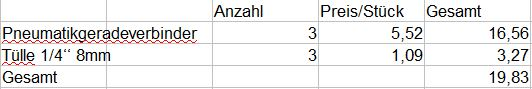
\includegraphics[width=\textwidth]{silas/preis}
    \begin{tabular}{|l|r|r||r|}
        \hline
        & Anzahl & Preis/Stück & Gesamt \\\hline
        Pneumatikgeradeverbinder & 3 & 5,52 & 16,56 \\\hline
        Tülle 1/4'' 8mm & 3 & 1,09 & 3,27 \\\hline
        Gesamt & & & 19,83 \\\hline
    \end{tabular}
    \caption{Preise von Schlauchzubehör}
\end{figure}


Die Entscheidung gegen die Steckverbindungsfittings
auf allen Seiten wurde wegen des Preises getroffen.
Der Preisvorteil liegt bei ca. 4 \euro{} und mit drei Teilen bei 12 \euro{} .
Die Schraubverbindungen sind alle nicht konisch ausgeführt. Dadurch sind die Verbindungen nicht selbstdichtend. Damit diese trotzdem verwendet werden können, wird Teflonband um die Gewinde gewickelt. Von den Tüllen werden die
Schläuche dann in die zu versorgenden Pflanzen gesteckt.

\subsection{Probleme bei der Realisation}
Bei der Montage und Realisierung sind einige Probleme aufgetreten. So hat der Schlauch nicht auf
die Fassung der Pumpe gepasst. Deshalb wurde ein Aquaristikschlauch mit einem
Außendurchmesser $12mm$ und einem Innendurchmesser von
$9mm$ genutzt. Die Fixierung erfolgte durch Schlauchklemmen, die an der Pumpe und am Übergang
zu dem Polyurethanschlauch für die sichere Verbindung sorgen. Ein weiteres Problem war das
Auffinden des passenden Kanisters. Herkömmliche
Kanister, wie zum Beispiel für destilliertes Wasser, haben eine Öffnung von $35mm$. Durch diese
Öffnung ist die Pumpe nicht versenkbar. Deshalb musste ein spezieller Kanister mit einer
Weithalsöffnung von $88mm$ besorgt werden.
Zusätzlich waren die Polyurethanschläuche nicht sehr flexibel, weshalb der Verteiler etwas
weiter entfernt platziert werden muss, um die erhöhten Biegeradien einzuhalten.

\section{Stromversorgung}

\subsection{Planung/Realisation}
Die erste grundsätzliche Frage, die zu klären war, ist, ob die Stromversorgung über ein Solarpanel
oder über ein Netzteil erfolgt. Deshalb wurden erstmal alle Verbraucher mit ihren elektrischen K
enndaten bestimmt. Zusätzlich wurde
die Betriebsdauer an einem Tag der Teile festgesetzt.


\begin{figure}[ht]
    \centering
    %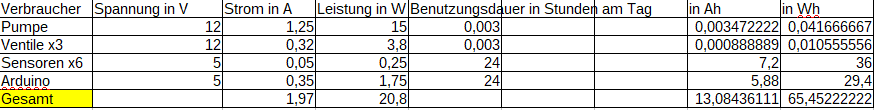
\includegraphics[width=\textwidth]{silas/verbrauch}
    \begin{tabular}{|l|r|r|r|r|r|r|}
        \hline
        Verbraucher & Spannung & Strom & Leistung & Dauer & in Ah & in Wh \\\hline\hline
        Pumpe & 12V & 1,25 & 15 & 0,003 & 0,003472 & 0,4166 \\\hline
        Ventile x3 & 12V & 0,32 & 3,8 & 0,003 & 0,00088 & 0,01055 \\\hline
        Sensoren x6 & 5 & 0,05 & 0,25 & 24 & 7,2 & 36 \\\hline
        Arduino & 5 & 0,35 & 1,75 & 24 & 5,88 & 29,4 \\\hline
        Gesamt &  & 1,97 & 20,8 &  & 13,0843 & 65,452 \\\hline
    \end{tabular}
    \caption{Stromverbrauch der Komponenten}
\end{figure}

Es gibt zwei Versorgungsspannungen.
Mit $12V$ wird das Arduinoboard versorgt. Um die benötigten Potentiale so gering wie
möglich zu halten, wurden die anderen Bauteile auch mit $12V$
Betriebsspannung ausgesucht. Nur für die Sensoren werden $5V$ benötigt.
Aus der Abbildung ist zu entnehmen, das die großen Verbraucher, wie die Pumpe und die Ventile,
nur die maximale Momentanleistung und damit den maximalen Momentanstrom festlegen. Für die
benötigte Gesamtleistung sind die dauerlaufenden Bauteile viel entscheidender.
Auf Basis der Leistungswerte und der Faustformel für
Solarpanels $W_{peak} * 4 = W_{tag}$ wird ein Panel mit mindestens $30W_{peak}$ benötigt. Das
hier eingeplante Panel \footnote{https://www.offgridtec.com/offgridtecr-30w-mono-$12V$-solarpanel.html}
bringt mehrere Probleme mit sich. So sind die
Abmessung von $340x605mm$ schwer in ein schlankes Gehäuse zu integrieren. Des weiteren sind die
Kosten wieder mitentscheidend. Für die Panellösung
muss zusätzlich ein Laderegler (ca.10-20 \euro{}) und eine Batterie(ca. 10-20 \euro{}) besorgt werden.
Im Vergleich zu dem dann letztendlich verwendeten Netzteil mit Kabel (21,25 \euro{}) liegt der
Preisnachteil bei ca. 45-55 \euro{}. Das Netzteilkabel liefert
durch eine Steckerbuchse den Strom an die Komponente. Die maximale Strommenge des Netzteil beträgt
$2,5 A$ und die maximale Leistung $30W$.
Da die Pumpen und Ventile mit dem Arduino geschalten werden, ist eine Schaltplatine notwendig.
Dazu kommt noch eine Platine, worauf die Spannungen zur Verfügung gestellt werden.

\subsection{Verteilerplatine}

\begin{figure}[ht]
    \centering
    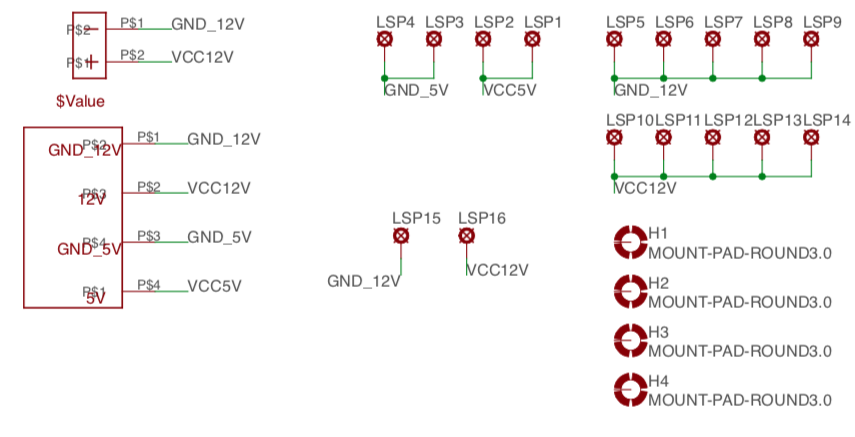
\includegraphics[width=\textwidth]{silas/verteiler1}
    \caption{Schaltplan der Verteilerplatine}
\end{figure}

In diesem Teil wird nur die Schaltungsplanung erläutert. Die Layouterstellung wird in einem späteren
Kapitel erklärt.
Die geplante Verteilerplatine soll die zwei Versorgungsspannungen zur Verfügung stellen.
Mittels eines DC-Jack werden die $12V$ von dem Netzteil auf die Platine geführt.
Von dort wird mittels eines DC/DC-Wandlers die Spannung auf $5V$
heruntergesetzt. Der Wandler hat vier Anschlussstifte. Zwei für $VCC$ $12V$ und $GND$ $12V$ und zwei
weitere für $VCC$ $5V$ und $GND$ $5V$. Von dem $5V$ Versorgungsbereich werden Abgänge zu der
Schaltplatine geplant. Ebenso gibt es Abgänge von dem $12V$ Niveau.
Die Masse des Netzteiles und der Platine sind durch den DC-Jack schon miteinander verbunden.
Zusätzlich wird die vom Wandler gestellte $5V$-Masse mit der Netzteilmasse verbunden. Dadurch
entsteht eine gemeinsame Masse und falsche Bezugspotentiale
werden ausgeschlossen. Auf jedem Potential wurde mindestens ein Reservelötloch eingeplant.
Das Arduinoboard wird über einen direkt eingelöteten DC Jackstecker versorgt.

\subsection{Schaltplatine}

\begin{figure}[ht]
    \centering
    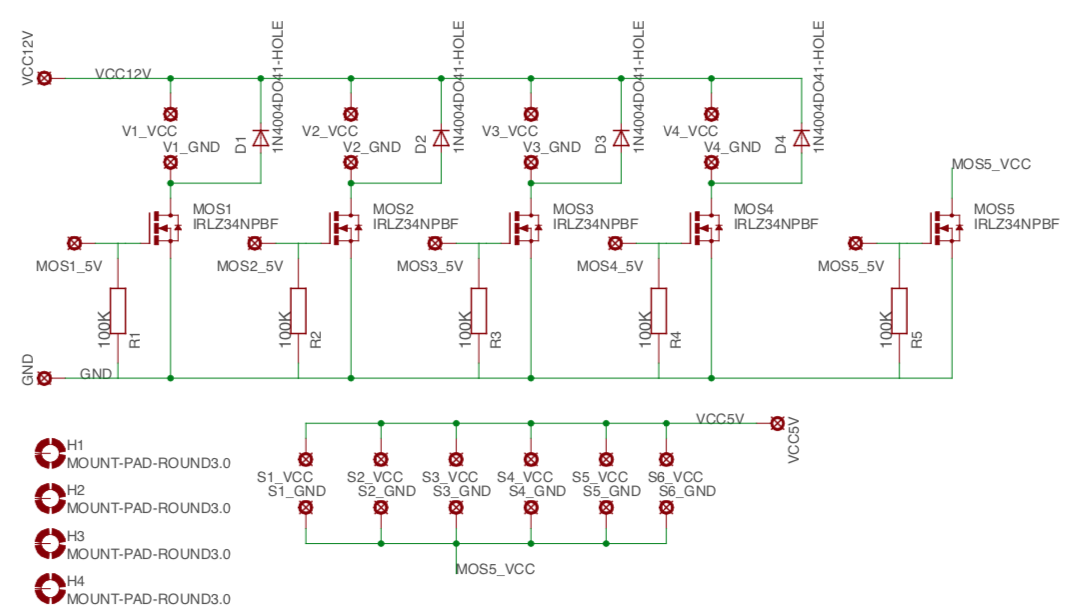
\includegraphics[width=\textwidth]{silas/versorgung1}
    \caption{Schaltplan der Versorgungsplatine}
\end{figure}

In diesem Teil wird nur die Schaltungsplanung erläutert. Die Layouterstellung wird in einem
späteren Kapitel erläutert.
Die Pumpen und die Ventile sollen durch einen Befehl des Arduinos einzeln an- und ausgeschalten
werden können. Die Sensoren sollen wegen Energiesparmaßnahmen gemeinsam ausgeschaltet werden können.
Als Schalter wird der Mosfet IRLZ34NPBF verwendet. Wichtig
ist, dass der Mosfet bei $5V$ Spannung durchschaltet und nicht höhere Threshholdspannungen benötigt.
Das Arduino kann nur $5V$ an den Pins liefern. Da induktive Lasten geschalten werden, muss eine
Freilaufdiode eingebaut werden. Darüber
baut sich Spannungsspitze der Selbstinduktion nach dem Ausschalten ab und schützt somit den Mosfet.
Parallel zu der Diode wird das induktive Bauteil eingesetzt. Die $100k\Omega$ Widerstände wirken
Pull-Down-artig. Damit wird garantiert das
der Mosfet immer sicher sperrt. Für die Sensoren wird keine Freilaufdiode benötigt,
weil hier nur geringe kapazitive Lasten zum tragen kommen.

\section{Gehäuse}
In dem Gehäuse soll die ganze Elektrik, Ventile un der Wasserverteiler verbaut werden.
Die Maße wurden durch die Biegeradien der Schläuche vorgegeben. Die somit ermittelten
Abmaße sind $350x300x100mm$. Als Material wurden herkömmliche Sieb-
druckplatten aus dem Baumarkt verwendet. Diese wurden zugeschnitten und mit Metallwinkeln
zu einem Kasten verbunden. Der Deckel wurde mit Scharnieren montiert. Die Ventile sind
auf Winkeln montiert und jederzeit entnehmbar. Der Verteiler
ist hingegen mit Schrauben direkt an der Bodenplatte befestigt. Für die Schläuche sind
Löcher mit $10mm$ Durchmesser in die Wand gebohrt worden. Diese Löcher wurden noch etwas
ausgefeilt, weil die Schläuche schwer durch zu bewegen waren.
Auf jeder Seite, wo schon Löcher vorhanden sind, wurden noch welche für die Leitungen gebohrt.
Auf der Zuführungsseite wurde das Leitungsloch größer mit $13mm$ Durchmesser, denn der Stecker
vom Netzteil wird durch diese Bohrung geführt.
Die Elektrik ist in einem Kunststoffkasten gekoffert. Der Kasten hat die Abmaße von $185x105x61mm$
und ist an den Deckel des Gehäuses festgeschraubt. Hier mussten auch auf zwei gegenüberliegenden
Seiten Löcher für die Leitungen gebohrt werden.
Auf der einen Seite ist die Stromzuführung und auf der anderen sind die Abgänge für die Ventile
beziehungsweise Sensoren.
\begin{figure}
    \centering
    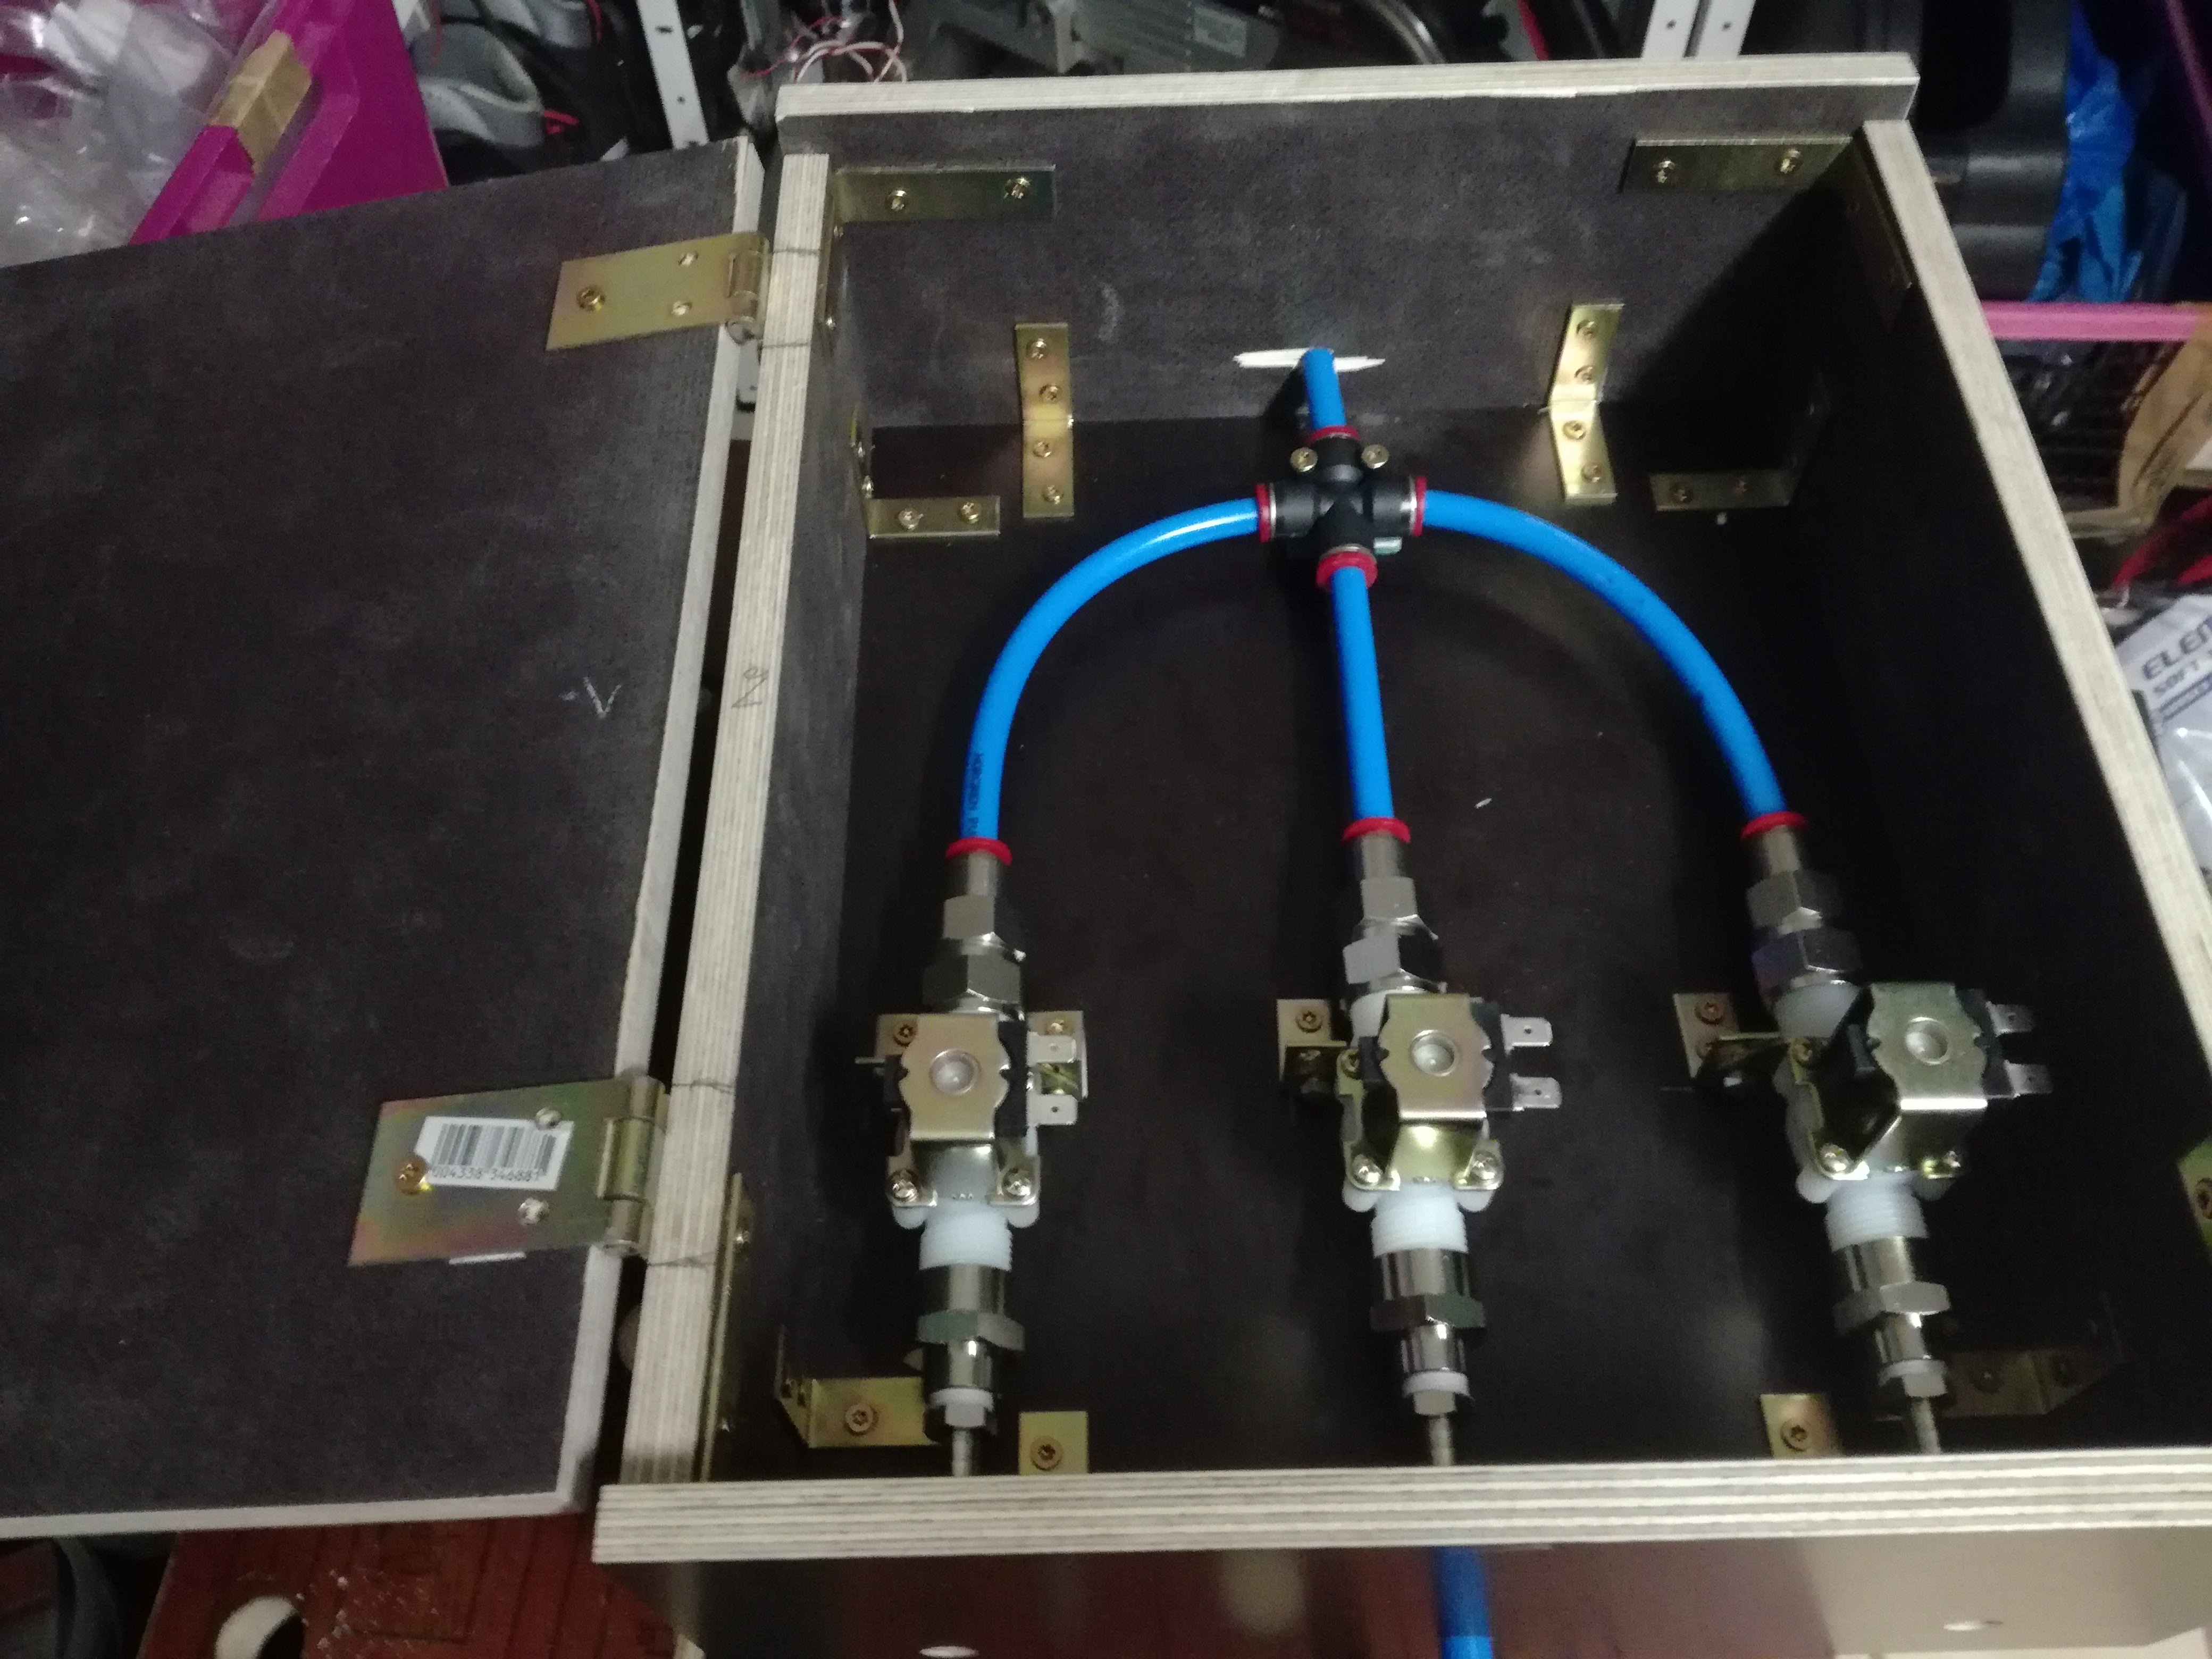
\includegraphics[width=\textwidth]{silas/gehause}
    \caption{Innenraum des Gehäuses}
\end{figure}